\subsection{ Overview Extending Dataset}

Extending the dataset is in a form of asking more questions about the objects found in EQA-MP3D. The new generated questions are size and spatial questions, and they are constructed in an episode form. The episodes, as mentioned in previous sections, are executable functions when inserted in an environment they yield an answer. In order to make a question-answer an executable episode-function, we copy the navigational \& object data of every episode in EQA-MP3D and generate new question for each unit of the nav data.


The questions' strings are automatically generated in templates. For each template of a question-type, there are two variants of the template. One variant with a room specified in the question and the other without specified room. The one with room specified are for generating a question of an EQA-MP3d episode of color\_room type, such that a question like "what color is the table in the room?" would have a corresponding size question "how big is the table in the livning room?". Templates with unspecified room are for generating new question of the episodes of "color" type in EQA-MP3D, such as "what color is the table?", and the new question would be "how big is the table?". 

The templates for size questions are as the following: 

size\_obj : 'how big <AUX> the <OBJ> ? \\
size\_room:'how big <AUX>  the <OBJ> in the <ROOM>?'  

Size question-episodes do not include the insertion of new object's info. Size question relies on turning a color question into a size one without the addition of other meta-data into the newly transformed episode. The object's info such as, center and radius of its AABB are taken as they are from an EQA-MP3D episode into a new episode. 

The spatial questions are of three relational types. A spatial question can either ask if there is an object "next to", "on" or "close to" other object. For each relational type there two variants of templates. The templates are the following: 

 '<AUX> there <ARTICLE> <OBJ1> close to the <OBJ> in the <ROOM>?'/\\
'<AUX> there <ARTICLE>  <OBJ1> next to the <OBJ> in the <ROOM>?' \\
'<AUX>  there <ARTICLE> <OBJ1> on the <OBJ> in the <ROOM>?\\
'<AUX> there <ARTICLE> <OBJ1> close to the <OBJ>?',\\
'<AUX>  there <ARTICLE> <OBJ1> next to the <OBJ> ?',\\
'<AUX>  there <ARTICLE> <OBJ1> on the <OBJ>?'

Spatial questions include the addition of a new object's info into an episode. The new object is the object used to question about a spatial relation with the already existent object in an EQA-MP3D episode. For example, a generated question as "is there a chair next to the table?" where "table" is an object in an EQA-MP3D episode and chair is a new object found within a relation to the table, and therefore, it has its data inserted in the new episode.



\paragraph{work organization}

The work structure of generating question consist of two components. The first component is a parser that does data extraction and processing, and has the functionality of acting as a calculator for measuring spatial relations. The second component is the question-answer episode generator. 

 
This section begins with describing the parser, then the question-generator and ends with presenting results. Description of the parser is split in two parts; The first part shows the process of extracting semantic annotations, and the second part views how the spatial relations are estimated. The section, thereafter, moves to describing the workflow of the generator, and the criteria in which the episodes of each question type is constructed. Finally the section ends with results showing the number of questions generated for each question type, and the answer distribution of the questions in the extended data-set. The results section ends with a discussion around the semantics of the questions asked. The discussion raises questions about the precision of the conveyed meaning in the question-answers, and how might the meaning be perceived. 


\subsection{Data parser}


The data parser is initially used to parse the semantic annotations and process geometric data and save it for the use of generating answers. The second functionality of the parser is to act as spatial relation estimator used simultaneously while generating questions. These two functionalities are are divided in two components. We begin with describing the first component, annotation extractor, which includes two different experiments/ways of extraction. The description of the second component, spatial estimator, includes the measurements in which spatial relations were determined for pairs of objects. 

The first experiment for extracting semantic annotation is through extraction from 'house files' of the MP3D data-set. The second experiment uses Habitat Simulator and sensors. The annotations extracted from the sensors in the Habitat's simulated environments provide additional computed information and slightly different raw data from MP3D annotations; In particular, some object names are different, but the rest of information, such as object ids and location-centers, is consistent with the annotation of the MP3D. 

In the existing generated question-answers data-set we use the data extracted through the Habitat semantic sensors. The main reason for choosing Habitat's simulator's sensors is because they provide a computed geometric information of the object's Axis Oriented Bounding Box. The MatterPort files include only the radius of objects' OOBBs.  An additional important reason for this choice of extraction is that some of  objects names output-ed by the sensors are aligning with the names found in the original EQA-mp3d data-set. For example, object names in MP3D such as l-shaped sofa and rounded-sofa are transformed, in Habitat's sensor, into their Hypernym category 'sofa'. Choosing object names that are aligning with names found EQA-mp3d, is helpful for having the overall data consistent with each other when we emerge our generated questions with EQA-mp3d. 



\subsubsection{Direct annotation extraction from MP3D files}


We extract two types of raw information from each object's line of annotation found in the house files in Matter-port. Lines mentioned erlier: [px py pz  a0x a0y a0z  a1x a1y a1z  r0 r1 r2 0 0 0 0 0 0 0 0 ] 

First we take the obj and room indexes (ids). Second is the [px py pz] and where we categorize it as the center of the OOBB of the box. Third is the [r0 r1 r2] (radius of the OOBB).

we structure the data in a form that the annotation of a house begins with the first level in it, followed by the rooms and objects in each room as: house 1 [{level1:room1[bedroom]:(obj1:bed,obj2:..),room2:(obj..)},, {level2:......} ]. The extracted data is then saved into a file. 

\subsubsection{Annotation extraction using Habitat Simulator}

Our final choice for extracting semantic annotations is Habitat's simulator. Our annotation's parser of the houses uses the sensors with configuration provided by the habitat platform \footnote{\url{https://aihabitat.org/docs/habitat-lab/habitat-sim-demo.html\#scene-semantic-annotations}.}. The configurations include the settings such as the scene, the height and width of the sensors, and the types of sensors to include. color sensor, semantic sensor and depth sensors are used. 

Once we simulate the environment, the sensors output the annotations of a house(scene) as an object. We iterate through the object to obtain information about the levels, rooms, and the objects in the rooms. We freeze the simulator once the annotations' object of one environment is outputted, then repeat the process for the other environments. 

In addition to the semantic annotation, we extract the center, radius of each of the AABB and OOBB of the objects. The radius size of the AABB is computed within the simulator and is streamed out with objects annotations. The radius of the OOBB is used for finding the objects' sizes. The center and radius of the AABB are processed into an information useful for a method of estimating spatial relations among objects. 

\paragraph{Calculating the Min and Max values of AABB corners}

The center and radius of the AABB are used to find position points on the edges of the object. Knowing the borders of an object's AABB provide a way to determine a spacial relation between objects given a criteria of distances between the corners of two objects . The first Information we obtain from the center and radius of the object is two corners of the AABB. Figure \ref{fig:aabb} illustrates an AABB in 3D as  the AABBs we get with the objects annotation. Each of $R_{x}, R_{y}, R_{z} $ is 1d radius on the x,y,z axis, where the  x is the length, y is the width, and z is the height. The radius in 3d would be the line/vector from the center (C) to either min or mix. 


\begin{figure}[H]
\centering
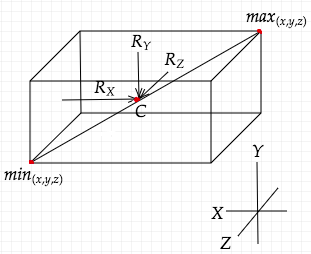
\includegraphics[scale=0.5]{images/Geoinfo.png}
\caption{Min and Max of an Axis Orients Bounding Box. $R_{x}$ is the radius on the x-axis, $R_{y}$ is the radius on the y-axis, $R_{z}$ is the radius on the z axis. The line from C to Max is the radius in 3D which is also equal to the line from C to Min. The line from Min to Max is the 3D diameter. Radius is half of the diameter.}
\label{fig:aabb}
\end{figure}

The first calculation is finding the 'min' and 'max' points of a bounding box given an object's center and its 3D radius. The min represents the corner point in the minus direction from the center in all the axis, and max is the corner on the positive direction from the center in all axis. 
%$\displaystyle
The AABB radius extracted from the habitat simulator is in diameter form as the line from min to max. The radius would be half the extent of the diameter so we get the 3D radius by simply dividing the the diameter by two. $ Radius = D_(x,y,z) /2\ $. 

The 'min' is the position point stretched from the center by the length of the radius on the negative direction of all the axis, and 'max' is the point on the positive direction of the center, at the end of the radius length. Calculating the min and max, is therefore, done by subtracting or adding the 3D radius from the 3D center. The center is a point at one ends of radius and the radius is a vector, if we add the length of the vector to the center point we get the point at the end of it's length "Max", and if we subtract the radius length from the center point we get point at the end of the radius length in the minus direction which is the "Min". Below, C denotes the center point and $\vec{R}$ denotes the radius as a vector.  
\[
Min\ point\ =\ C\ -\ \vec{R} \ \ =\ ( x_{1} -x_{2}, y_{1} - y_{2} , z_{1} - z_{2}{}) \] 
\[
Max\ point\ =\ C\ +\ \vec{R} \ \ =\ ( x_{1} + x_{2}, y_{1} + y_{2}, z_{1} + z_{2}{}) \ 
\]

The min and max as corners of the box could be used to estimate distances between objects. For example, in 3D game design they are often used for collision detection. From the Min and Max one could the values of all the other corners, as the values of the other corners range between the [Min,Max] on all the axis. In the following sections we describe in detail how the Min and Max used in a technique for finding spatial relations between objects. 

For every object in the annotation we find the Min and Max of its AABB and extract the radius of its OOBB. The radius of OOBB is given with the data extracted in the simulator. We use the OOBB radius for calculating the sizes of the objects. We consider the size as the volume of the box which is the length multiplied with the height and width. In our case the length is the x delimiter, width is the y delimiter and height is z delimiter. The calculated volume of a box is \begin{math} X\ x\ Y\ x\ Z \end{math}. 

\paragraph{Storing the annotations}

We structure the annotations and save them in a file. The structure of the data consist of a dictionary storing the data in a hierarchical way. At the top part is the house id, then rooms in the house, then the objects in the house. Each object stored by id, contains the Min and max value of its AABB, radius of the OOBB, its name \& ID , room name, and the level id where the room is located. Structuring and processing the data and having it stored in files allows to access all the objects in a room through the scene id and room id, which accelerates the question generating process.  

We store the calculated volume of each object in all the houses and store it in a second file. The volumes of objects are stored by their object category. In the volumes file, we find the volumes of all the objects in all of the houses stored in a dictionary, each key represents a category such as 'sofa' with values of the volumes of this object type. The point here is to obtain data on the sizes of each object type. We use this information for finding ground truth answers about for the size questions. Defining answers for size questions is elaborated in detail in further sections. 
 

\subsubsection{Spatial relation estimator}

The functionality of the estimator is to take a group of objects and pair them according to spatial relations. We give the estimator all the objects in a room to find pairs that are 'on', 'next to' or 'close' to each other. If the mentioned relations are founded between two objects, the pairs are organized in a dictionary, one key for each spatial relation. This information is used for generating positive spatial questions. 

The first measure for determining the mentioned spatial relations is by calculating the distance between the corners of AABBs of two objects. In the processed annotations the objects are initially represented by two corners, 'min' and 'max', as seen  previous section. The other corner points of the box can be extrapolated from the 'min' and 'max', as certain dimensions overlap. 

\paragraph{Extrapolating AABB corners from Min \& Max Points}

In figure \ref{fig:box_points} illustrates the eight corners, the view point of the cube is rotated to the right for the sake of viewing all the points in the cube. If we move our point of view directly in front of the cube as if  we are facing the square GHED,  the points A and H would seem to be lying on a straight line. Lying on the same straight line, for example, means the point A and H are located on the same points in the x-axis, and so one for the other parallel points. 


\begin{figure}[H]
\centering
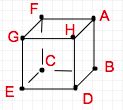
\includegraphics{images/cornerPoints.png} %[scale=0.5]
\caption{Corners of Axis-Aligned Bounding Box. The box viewed here from upward rotated to the right position in relation to the front of the box. The correct global viewpoint of the box would be by imagining our viewpoint straight facing the square GHED, where A\&H would be on a straight line(simiar points on the x-axis), and as such for all other parallel points. From the illustrated corners A would be the 'Max' and 'E' would be the min}
\label{fig:box_points}
\end{figure} 

We get the rest of points from the Min and Max of an AABB for the reason that AABB's are not rotated and aligning with the global view. To express it better, we image the global point of view of the AABBS as a view facing a group of adjusted and not rotated boxes. When the axis are aligned, the values of the corners would overlap where the 3D values on the (x,y,z) would be either the 'Max' or 'Min' in each dimension. For our example in figure \ref{fig:box_points}, the point \textit{A} represents the  "Max" corner point, and the point  \textit{E} represents the "Min" corner. We can extrapolate, from the 'Min' \& 'Max', the six other corners as such:   
$\begin{array}{l}
A\ =( x_{max} ,Y_{max,} Z_{max}) ,F=\ ( x_{min} ,Y_{max,} Z_{max}) ,H\ =\ ( x_{max} ,Y_{min,} Z_{max}) ,\\
B=( x_{max} ,Y_{max,} Z_{min}) ,D=\ ( x_{max} ,Y_{min,} Z_{min}) ,\ C=( x_{min} ,Y_{max,} Z_{min}) ,\\
G=\ ( x_{min} ,Y_{min,} Z_{max}) ,\ E\ =( x_{min} ,Y_{min,} Z_{min})
\end{array}$


\paragraph{Measuring the distance between AABB corners}

The first criteria for determining a potential pair with spatial relation is the distance between their corners. The Euclidean distance between two corner points; denoted as the distance between p and q, where P is one corner of an object and q is corner of other. \textit{n} denotes an Euclidean space,   $q_{i} \& p_{i}$ are the Euclidean vectors of the corners where the base \textit{i} stand for the dimensions of the vector. The formula can be described as the square root of the sum of the square of the subtractions of q and p at every \textit{i}-dimension. 

\[
 d\left( p,q\right)   = \sqrt {\sum _{i=1}^{n}  \left( q_{i}-p_{i}\right)^2}
\]

The corners, depending on the type of relation we want to extract, can be represented as points in  1d, 2d, or 3d. For example, to filter pair of objects where one is 'on' the other, we would check how close they on 3D axis but then we want to know the distance on z-axis(the height) in particular; Therefore we would calculate the euclidean distance for the corners in 1D as such: $ \sqrt{ (z_{1}-z_{2})^{2}}$. Knowing the distance on the x and y axis would be an indicative of corners next to each other in this case we measure the distance of 2d corners and such:$ \sqrt{ (x_{1}-x_{2})^{2}+(y_{1}-y_{2})^{2} }$. We would represent the corners in 3D if we would want to measure how close two corners to each other in general, not on a specified axis. The Euclidean distance between two 3D points would be as such: $ \sqrt{( x_{1} -x_{2})^{2} +( y_{1} -y_{2})^{2} \ +\ ( z_{1} -z_{2})^{2}\ } $

\paragraph{Classifying relations between the sidelines of AABBs}

If a pair of objects are close in distance, we distinguish the possible spatial relations they have depending on the overlap of their sides of their AABBs. For example, close boxes that might be 'on' each other, the vertical line (Z(max),Z(min)) of one object should be contained within the vertical line of the other, otherwise, this would mean the one is inside the other instead of being on it. This measuring criteria is intended to check for possible spatial relations among the pairs with close distance. This technique is used in different instances while determining if an object is "next to" or "on"



\begin{figure}[H]
\centering
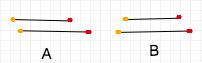
\includegraphics[scale=0.5]{images/contained.png}
\caption{Text to be added}
\label{fig:contained}
\end{figure}

The calculation if one side is contained within the other relies on defined criteria. The calculation is done in a specific function and  can take as input  corner points on one axis or more. In the drawing \ref{fig:contained} 'A' represents two lines on the 'X' axis where the top part is not contained within the other, an in 'B' the top is contained within the lower line. In this example we determine the 'contain' relation by taking the 'min' represented by the the orange dot and the 'max' doted in red. 

If the min of the upper line is greater than the min of the lower line and the max of the upper line is less than the max of the lower line then the upper line is contained within the lower. Hence the 'min' of the upper line is greater than the 'min' of the lower line because it's more to the right in the positive direction of the 'x' axis. If the previous condition is not satisfied, then the lines are otherwise not contained. 

The operations above are done over different axis for every relation. Below we specify how each of the 'on', 'next to', and 'close' relation is determined between the objects. 

\paragraph{On}



First step is choosing pairs of objects that are closest to each other vertically(on the Z axis). The distance should be less than a 0.5 millimeter thresh hold. The Euclidean distance here is calculated between the 1D points on the Z axis only. Two corner values from each box and any corner match the distance required are picked out. 

\begin{figure}[H]
\centering
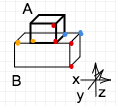
\includegraphics[scale=0.7]{images/on.png}
\caption{Text to be added }
\label{fig:on}
\end{figure}


The second step consist of a group of conditions that the pair of objects need to meet in order to be considered on each other. The first condition is that the vertical sides, the line from Zmin to Zmax, of the boxes are not contained within each other. The Zmin-Zmax lines of every object box are the lines between the two red dots in box A ans B in the illustration \ref{fig:on}. Otherwise if the lines on the Z axis are contained it would mean one object is inside the other. 

The second condition is that the horizontal line of one of the boxes is contained within each other.The horizontal lines in the illustration are from the Orange to the red points in each box. The lines on the y axis from the red to the blue points should also be contained. 

The final step is deciding which object is on the top of the other. The pair of objects are passed to a function that see which Zmin-Zmax has greater value. The object on the top should be in the upward positive direction. 


\paragraph{next to}


\begin{figure}[H]
\centering
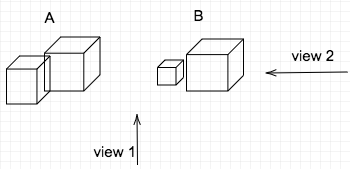
\includegraphics[scale=0.5]{images/Nextview.png}
\caption{To be replaced by new figure}
\label{fig:next}
\end{figure}


A pair of objects next to each other have to have a distance not greater than 0.1 meters on the X and Y axis. The distance here is calculated for 2D corner points, this means the distance is calculated for four corners (min and max front and back).

The pairs should not have contained sides in neither the x nor the y axis. In this condition a pair of objects next to each other would like illustration A in \ref{fig:next}. This is might a bit different from what we consider next to each other as humans. We might imagine a typical next to pair as illustration B seen from view 1.

However, the choice of having 'next to' pairs not contained with each other is due to considerations of the view point. From view 1 the pair(B) seem next to each other but from view 2 they would not. In pair(B) from view 2, one object would be behind the other and likely hidden. So if view 1 is the global view and we pair the objects as in (B), seen as next to in view 1, the robot might enter the scene from view 2 and it would be wrong to refer to the pair as next to each other. However, if the 'next to' pairs are assigned as in illustration (A), the pair would be still visible in whichever view, and positioned proper enough to be referred to as next to each other. 

Finally the pair must have their lines contained on the Z axis. Otherwise, the two objects might satisfy the first condition on the (x,y) but be distant on the z axis, such as one object in the ceiling and the other on the floor. 


\paragraph{close to}

A pair close to each other are a pair who has any of their 3D corners close to each other within a max distance of 0.2 meter. No other conditions required for the pairing of objects close to each other. It can be a close object on, above, below or next to. 

\subsection{Second Module - question generation (To be reviewed)}


\begin{figure}[H]
\centering
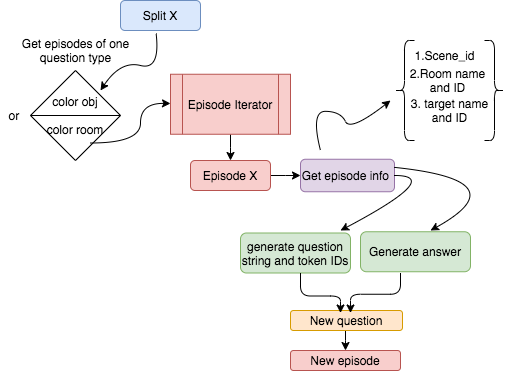
\includegraphics[scale=0.5]{images/generator.png}
\caption{Split generator}
\label{fig:generator}
\end{figure}



 Our question generator generates questions of two types, size and spatial. In order to run the generator, the arguments required are the type of question, path to the val and train splits. 


 The question generator generates questions of one type at the time. Questions with the string "room" in is considered a different type from a question that refers to objects without a room. For example, the question "How big is the table?" has the type "Size", and the question "How big the table in the living-room?" is of type "Size room". In order to generate size questions with and without reference to a room, therefore, requires ruining the code, one separate time for each type. 

The split generator is the core component in the code. It takes a split either train/val and a question-type as arguments. The functionality of the split generator is to turn an EQA v1 split of episodes into a new split of new episodes. In figure \ref{fig:generator} we see an illustration of the workflow of the split generator. The five general steps is filtering(uncolored rotated square), iterator(red rectangle), episode parser (pink rectangle),  QA generator (the green rectangles), and  episode wrapper (the bottom yellow rectangle- inputs QA and outputs episode )  

The filter returns a set of question-episodes of one type only. The returned set of questions of a type is dependent on the question type given to generate. For example, if the input is to generate questions of 'size-room', 'how big is the sofa in the room', we take only the questions of "color-room" type. 

The filtered set is passed to an iterator. Each iteration passes one episode from EQA-v1 to a parser. The parser function in the iterator extract information, such as the object name and id, scene ID and room ID, from the EQA-V1 episode. 

The parsed information is passed to a QA generator. The QA generator is better described  as a group functions of the split-generator that are conditioned differently dependent on the question type. The answer generation function is, however, a different function for each question type.  

 The general idea for generating QA of any type relies on two straightforward steps. First, generating a ground-truth answer for the given question, which is the most important stage in the generation process as it requires calculating values from the data in the houses. Second step generating a question string and token ID's.

The  final step consists of inserting the new question with the corresponding geometric information, and structuring them into an executable function.  We call a QA sample an episode when the section of the episode seen in figure \ref{fig:episode} are filled with the new QA and the other the corresponding information. 

Our question generation can be described as generating one question for every “shortest path” there is. The idea of transforming  an episode from EQA into a new one is based on using the starting position and the 'shortest path' found in them. Having more questions for each shortest path is equivalent to having multiple questions about the same scene. 

\begin{figure}[H]
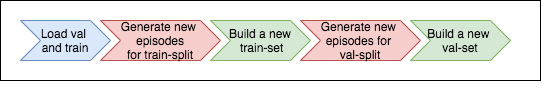
\includegraphics[scale=0.5]{images/stages.png}
\caption{Split generator (The top part of the code)}
\label{fig:stages}
\end{figure}


The top most part of the code (the data-set generator), illustrated in figure\ref{fig:stages} , passes the train and val to the split generator at different time-stamps. The reason for generating the two splits in two different stages is to keep track of the number of question-answers generated for each split. Emerging the two splits and splitting them randomly at the end might create and imbalance between the  answers in each split. The current code controls the distribution of answers in the train and val sets. Otherwise, leaving the type of answers uncontrolled would leave a bias towards one answer over the other. 

Once a split of episodes is generated it's passed to loader function. The loader function inserts the answer and question vocab to finalize the data-set in the form seen in figure 2.2

 In the coming two sub-section we describe in detail how the QA generators for the size and spatial questions work. 

\subsubsection{size-questions}

Size questions are generated through three steps. The first step is generating a ground truth answer about the size of the the target-object found in EQA-V1 episode. There three possible answers are  Big, Small, and Medium. The second step is generating a question string and token ids. The final step consist of filling the question-answer in an episode form, with shortest path and the rest of object's info from the original EQA-v1 episode, as described in the previous section. 

\subsubsection{Size answer} 

The size answer is generated in a function referred to as "GetsizeAnswer". This function takes as an argument the target-object's name and the size of its box and returns an answer about its size. The function calculates the volume of the target object in a similar way as the rest of the sizes of the objects. Volume of the OOBB = W x L x H. The next step in the function is to compare the size of the target to the sizes of the objects of its type.

The relative size is determined by its deviation from the standard of its type. As mentioned earlier the sizes of all objects are stored by type in a file. We pick the volumes of the object's type and calculate the mean size and the standard deviation of all the the sizes from the mean. The standard deviation denoted below: 

\[ s = \sqrt{\frac{1}{N-1} \sum_{i=1}^N (x_i - \overline{x})^2} 
\]

The answer is 'small' if the objects' size is smaller the mean size of its type minus the standard deviation,  'big' if the size is larger the median + the standard deviation, and middle if the size of the object is within the standard deviation added and subtracted from median. 

We control the answers' distribution. We observe that a majority of objects have a medium size given the standard of their type. In order to avoid bias towards the 'medium' answer, we restrict the number of QA with medium answer. We keep track of how many QA with medium answers has been generated and when the number reaches a limit we generate None QA that are later filtered out. The limit varies depending on the question type and the split (train or val), and is based on our observation of the answer distribution in the splits. Note that we refer to 'question type' in this example if either the question to be generated is size question with string 'room' such as "color-room" or without. 



\subsubsection{spatial-questions}

Generating spatial question takes more complex steps and longer time than generating size questions. Generating a spatial QA requires a coordination with the spatial relation extractor. In addition, spatial questions include the addition of an extra object to the question string, and the insertion of the new object's information into the QA episode. 

Searching for spatial relations of the target object in an EQA episode is the first step taken. We pass the scene an room id to the 'relation' extractor to obtain pairs of objects, within a room,  with a spatial relation between them. The relation extractor returns three types of relational : next, on, or close, if existent within a room. Else it returns a category with empty values. 

The decision of generating a question of one of the mentioned relational categories is dependent on the existent of an object with a spatial relation to the target object. The process of executing a generation command of a question of a spatial type is illustrated in figure \ref{fig:spatial}. If there is an object 'on' the target or a target is on another object, we generate one questions, and similar case if there is an object next to the target object. If there is no 'on' or 'next' relation or either of them is non existent, the criteria for checking if there is a 'close' object is satisfied. If none of the conditions are satisfied a QA with no 'answer' of a random spatial type is generated.   

\begin{figure}[h]
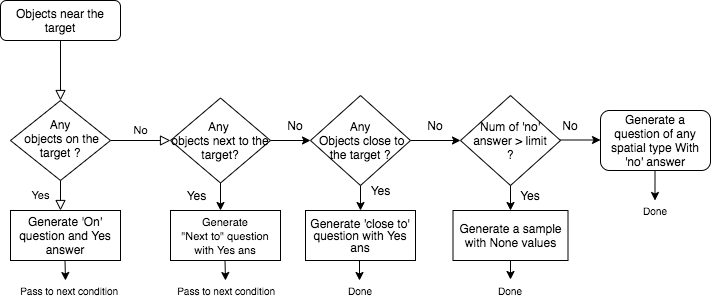
\includegraphics[scale=0.4]{images/spatialconditions.png} %[scale=0.2]
\caption{Decision tree for generating different types of spatial questions}
\label{fig:spatial}
\end{figure}

A QA with positive spatial answer has a 'yes' answer, and 'no' if a relation is non existent. The decision tree as seen \ref{fig:spatial} leverages positive QA for the reason that we observe that the no-relation instances outnumber the positive ones. The final condition, we even control the number of QA with 'no' answer by generating a None QA if the number of generated QA with no answer reaches a limit. The QAs' with None values are later filtered out.

Within this decision structure, for each 'shortest path' in an EQA episode, there is a possibility for generating from one to two spatial questions of different spatial type. 

The process of generating a spatial question includes the addition of information about two objects. An episode/question generator, a group of functions, adjust itself to a spatial question generation if certain arguments are given to it. These arguments are seen in the input section  in the illustration in fig \ref{fig:spatialGen}. Such as potential  object type, spatial question type, and all object in a room 

\begin{figure}[h]
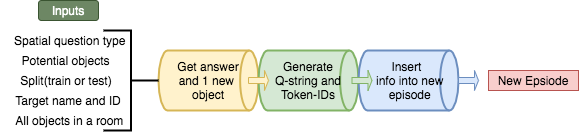
\includegraphics[scale=0.4]{images/spatialGenerator.png} %[scale=0.2]
\caption{Structure of spatial questions generator}
\label{fig:spatialGen}
\end{figure}

All the inputs seen in \ref{fig:spatialGen} are required to generate an answer from a function called "GetSpatialAnswer". All objects in a room are needed for generating "no" answer. In case of generating a "no" answer the "GetSpatialAnswer" function picks a random object fro the houses that is not in the room. The reason of excluding objects in the room from the selection of a random object for a negative QA is to help us in the validation process, such as we would know if the robot answer 'yes' to a QA with 'no' as ground truth that it's due to bias rather than he robot recognizing the object in the scene. 

A selected object of potential objects and the type of spatial question are required arguments for generating spatial question string and token ids. 

The last part in blue is conditioned by the type of answer, if it's 'yes' or 'no'. If the answer is yes, geometric information of the target object's pair is passed to it to insert it in the episode. If the answer is 'no', no additional information is added to the episode beside the information of the target object found at the end of the shortest path. 


\subsection{Results}

\subsubsection{Total number of generated questions}

\begin{figure}[H]
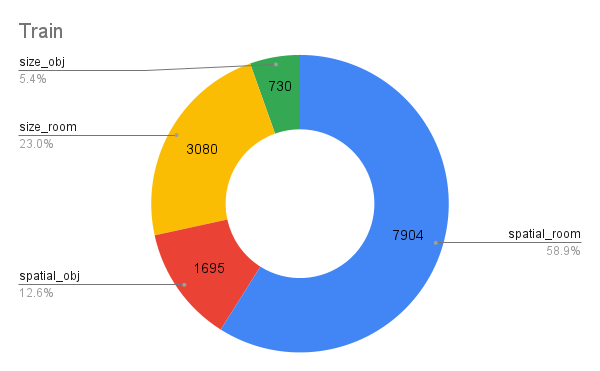
\includegraphics[scale=0.25]{images/GenTrain.png}
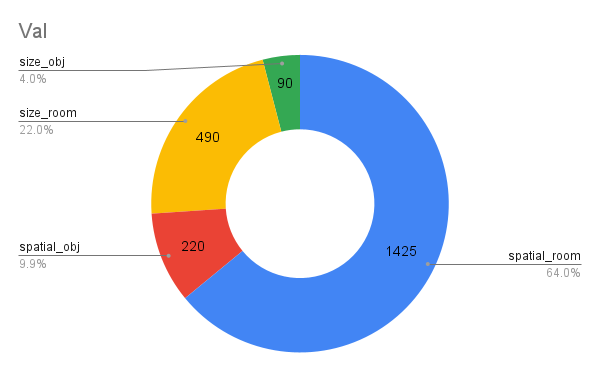
\includegraphics[scale=0.25]{images/GenVal.png}
\caption{}
\label{fig:questionGen}
\end{figure}

We generate a total of 13 409 question for train and 2 335 questions for validation.  In figure \ref{fig:questionGen} questions of size\_room and spatial\_room refer to questions that contains a reference to a room, such as 'How big is the bed in the bedroom?'. Questions of spatial\_obj or size\_obj type are questions with a reference to object only, such as "Is there a chair next to the table?". 

\subsubsection{Answers distribution}

\paragraph{Answers distribution of spatial questions}

\begin{figure}[H]
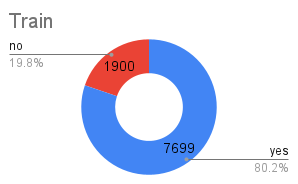
\includegraphics[scale=0.45]{images/TrAnSp.png}
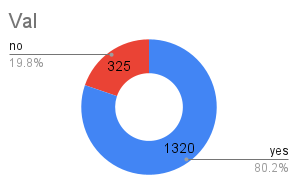
\includegraphics[scale=0.45]{images/VlAnSp.png}
\caption{}
\label{fig:AnsDist}
\end{figure}

The majority of answers for the spatial questions are positive "yes" as seen in figure \ref{fig:AnsDist}. This imbalanced distribution is an intended outcome. The motivation behind this intention is based on an idea, formulated by \cite{regier1996human}, of learning of positive samples only. The argument behind this approach to learning  is inspired from a cognitive theory of human's first acquisition of language. The theory is  based on the premise that humans tend to learn spatial relations from positive evidence instead of non existent instances.

\paragraph{Answers distribution of size questions}

\begin{figure}[H]
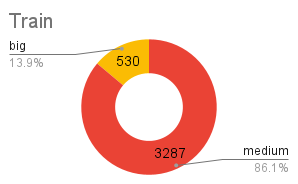
\includegraphics[scale=0.45]{images/TrAnSi.png}
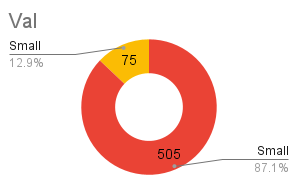
\includegraphics[scale=0.45]{images/VlAnSi.png}
\caption{}
\label{fig:AnsDistSI}
\end{figure}

The outcomes of generating size questions resulted with zero samples of "small" answer and a majority of 'medium' answer as seen in figure \ref{fig:AnsDistSI}. In the QA generator, we intended to limit the question-answers with "Medium" answer based on an observation of their dominance. However, limiting the 'medium' answers more than the presented numbers would have resulted in a very few question-answers of size type. An insignificant proportion of size questions was insufficient for training the model . We decided to keep the size questions with their imbalanced distribution, despite knowing that this linguistic bias might hinder the learning outcomes.  

Our question-answer generation is very dependent on the objects and the shortest paths found in EQA-V1 data-set. The geometric information such as  starting positions and shortest paths are required material for extracting scenes training and testing the VQA model. To be only dependent on the objects found in the EQA restricts our choice over the QA that we could generate. The most prominent limitation we see in the generated questions is the inability to control the answer distribution for size questions. None of the target object's found in EQA V1 turned to be of a small size, based on the criteria we establish for describing an object's size. 


\subsubsection{Discussion - (two paragraphs to be added)}

The description of sizes is paradoxical. A well known paradox in philosophy, the sorites paradox, uses the description of a "pile of sand" to display the dilemma of describing the size of an entity. The paradox, described by \cite{fisher2000sorites},is stated as such: is a grain of sand a pile of sand? No. does adding one or 5 or 20 grains make a pile of the sand?, the answer is still no. We can make inference that adding grains of sand does not make a pile. However, this inference is inaccurate because we might conclude that adding 10 million grains does not make a pile of sand, which is false. This is the reason why it is a paradox. A paradox is when the premises entail a logical inference but a conclusion we draw is false (\cite{fisher2000sorites}, \cite{sainsbury2009paradoxes}).

Sorties paradox can be expressed more clearly in prepositional logic, \emph{modus ponens}. \emph{Modes ponent} is a form deductive argument for making an inference. Its rule is based on conditionality of the truthfulness of a statement, if P is true then Q is true. The inference we make from making a pile is that, if "one grain of sand is no pile" is true, then "2 grains of sand is no pile" is also true. We denote the predicate 'no pile' as \emph{P}  and a grain of sand as \emph{a} and the number of grains as \emph{n}; one grain of sand makes no pile is the denoted as such $ P_{a_{1}} $, "two grains of sand is no pile", $  P_{a_{2}} $ , and our conclusion that adding any number of sands is no pile would be $ P_{a_{n+}} $. The process in which we made the inference ($ P_{a_{n+1}} $) adding more grains makes no pile is represented as such: \[ P_{a_{1}} \rightarrow \ P_{a_{2}} \rightarrow \ P_{a_{3}} \rightarrow \ P_{a_{4}}.... \rightarrow \ P_{a_{n+1}} \] if one grain of sand is no pile then two grains of sand is no pile, if two grains is no pile then three grains  no pile, if three grains is no pile then four grains is no pile, then we make the inference that adding any number of grains is no pile. The conclusion is  any number of grains do not make a pile. 


Paradoxical predicates are vague form of knowledge. The sorties paradox applies to all the adjectives and forms of expressions that lack a precise form of logical construct; Small, big, bold and expensive are examples of predicates equally paradoxical as the "pile" of sand \cite{kennedy2007vagueness}. From an epistemic approach, some philosophers disregard these forms of language expressions as valid arguments/knowledge about the world. In epistemology the questions in interest are how do we know what we know?, in what way was a certain knowledge obtained?. For example, how do we know that a pile of sand is a pile of sand or that a chair is a big chair not a small one; note that the knowledge of 'big chair' or 'pile of sand' is here the 'meaning' of them, what does the symbol "big chair" mean.\cite{williamson2002vagueness} notes that vague predicts distinguished from other predicates by the absence of a precise/clear boundary lines that separates their meaning from its negation, for example, the boundary line of when a pile is a pile and when it's not, or the boundary between  pretty and ugly, big and small. On the other hand The distinction between an animal and a tree has a clear borderline, one is inmate and the other is not. 

Paradoxical expressions are rejected, in the epistemic view, based on the unfounded precise reasoning that logically defines them. They are considered vague primarily for the absence of higher meaning of measure. The induction to explain what a 'pile'  means (in terms of properties of grains) proved to be paradoxical in classic logic, as seen in a previous example. The missing boundary of vagueness in classic logic is the distinguishing line of their truth-value, the one that separates True from false. 

\cite{williamson2002vagueness} quotes J.L Austin (\cite{austin1962sense}) on an argument regarding the usage of expressions such as 'accurate','precise', where J.L Austin disputes ,‘If I measure a banana with a ruler, I may find it to be precisely 5 5/8 inches long. If I measure my ruler with bananas, I may find it to be exactly six bananas long, though I couldn’t claim any great precision for my method of measurement’. One might say that our measurement of the banana is very precise, but to measure the truthful validity of our measurement is as accurate as measuring it with bananas. In the discussion found in (\cite{williamson2002vagueness}), vague expressions are seen in the epistemic view as a type of ignorance. 

It is important to stress that 'vague' refers to the representation of the entity (the description) not  the nature of it. Nature is logical, the world either exists or does not exist, the 'pile' exists regardless the vagueness of our measurement of its existence.  \cite{williamson2002vagueness} on Bertrand Russel's reference to vagueness, in  (\cite{russell1923vagueness}),  notes that Russel considers the issue of vagueness as a problem of symbol representation. \cite{quine2011two} refers to the distinction between the symbol representation and the symbol referred to in the world as intention and extension. Intention is the expression/representation/language we use to refer to an existent entity in the world, extension is the entity with its inherited property in the world as it is. Crescent/full moon are intentions, the extension is the same moon object as it is in the world. \cite{quine2011two} elaborates on Russel's assertion to vagueness as an issue with the intentions we use to describe the extension. \cite{williamson2002vagueness} points out the Russel means representation also in extra-linguistic properties, such as the perceptual representation we have of the extension. 

Sorties paradox reveal vague expressions of an ordinary language through a logical system of an ideal language. \cite{williamson2002vagueness} on Russel's assertion, in (\cite{russell1923vagueness}), that the existence of vague expressions indicates that language as a whole is vague. An ideal language must have a logical representational unit for every extension \cite{quine2011two}. Russell's then invalidates classic logic as suitable to express ordinary language (Ordinary language has vague, general,ambiguous expressions). In the debate whether logic could be used to explain vague expressions, \cite{williamson2002vagueness} cites Max Black (\cite{black1937vagueness}), responding to Russel's invalidation of logic in regard to vagueness, that Russel's claim is an evasion of responsibility to  describe natural language in systematic way. Black goes on in explaining that the incoherence of vague expressions in logic stems from a trouble that occurs by trying to logically formulate an expression of degree of truthiness without having explicit degrees of truth.  For Black, some expressions in ordinary language cannot be confined to absolute truthiness or falseness, they instead could be neither true or false. For example, we can say a person is not tall but somewhat tall, or that adding 3 grains don't make a pile but adding thousands of them could, so 'adding grains of sand makes a pile' is neither false or true but partially true. 


Supervaluation logic and  solutions for expressing vagueness. Super valuation suggests a three valued truthiness. An expression can be either super-true, super-false or undefined. For a statement to be super-true or super-false a condition must apply to all of its valuations; valuation can be, for example, the \emph{n} number of grains. A statement has "undefined" truth value if it has true valuations and false valuations. This three valued logic allows to distinguish precise expressions from 'borderline cases'(vague expressions). The obtaining of truth value of each valuation of the predicate is referred to as precisification. Precisification are referred to using quantifiers, existential quantifier $ \exists $ to refer to a single valuation ,  and universal quantifiers  $ \forall $ all the valuations. The logical statement below denotes that there exists an \emph{n} that's a border line for 'is no pile' where \emph{n+1} is a pile. The statement  draws a dividing line where at \emph{n}th grain, every \emph{n+1} after the line "is a pile" $\neg P( n_{+1}) $ 

\[ \exists n( P( n) \ \&\ \neg P( n_{+1}) \ ) \]

Despite the distinction of  borderlines in super-valuations, a deficiency in meaning, referred to as highr-order vagueness, still appears. If the borderline \emph{n}th , for example, is 8,000,000 grains of sand where all \emph{n+1} "is a pile", but isn't 8,999,99 also a pile?. This a sort of paradox that found initially. Also the difference between  very tall and tall would be still vague, the two predicates would fall after the dividing line with undefined difference. 


Fuzzy logic and fuzzy sets proposes a solution of truth range that lies  between [0,1]. This range of true values allows to map gradable matters, such as the difference between very short, tall, and very tall. Fuzzy sets maintains a feature of classical logic, that the absolute truth still lies in exclusion of a middle, [0,1],false or true. The range of turthness can be expressed in set theory using notions of intersection, union,
complementation and subset which correspond to conjunction, disjunction and negation. In set theory we can denote that a 'definitely is a pile' is distinguished from 'is pile' in a way that 'definitely is a pile' is a subset of 'is pile' without claiming that a pile is a subset of definitely is a pile'.  For example,  A is a set for 'definitely pile', and B is the set of 'is a pile', the relation can be expressed as $A\subset B $ (A is a proper subset of B), where all the elements in A are in B but B has more elements that could be for example, "is kind of a pile". 

Sets can be formed in Boolean functions with conditions which makes it very flexible for usage in computer applications and programming languages. (\cite{williamson2002vagueness}) asserts that the development of fuzzy logic out of fuzzy sets allows for a replacement of [0,1] to any established range of number, for example we could say that \emph{n} is a member of the 'is no pile' set (C) if its value is 0 or more and less than $10,000:  n \in  C  If  0≤ n< 10,00.$

\paragraph{Vague descriptions of sizes}

For size questions,the object is considered an element of a size set if its within the range assigned for the set. The range and borderlines of each set are determined in relation to a context. Establishing a range for a vague expression relative to a context is defined by (\cite{raffman1996vagueness} ,pp 181) as  multi-range theory 

"For any object O, vague predicate 'P', and total context TC:
'P' applies to O, relative to TC, just in case a competent
speaker could judge O in TC and, were he to judge it in
TC, he would apply 'P' to it."

The context in this project has been defined by the category of objects found in all the 3D environment; For example, the context of "big sofa" is all the sofas we find in MP3D. The standard deviation can be seen as the established boundaries taken from the contexts. The range of deviation of each object category is different and respective to its context, so that the size range of "big sofas" is different from the range of "big fireplace". The ranges stretch from the mean on the minus or plus as mentioned in section ..


The followed approach attempted to reduce vagueness following the semantic conventions for dealing with vagueness. However, even if semantics manage to find logical means to express vagueness as clear as possible, in an epistemic view this clarity is still in question. Semantically, perhaps the burden of clarifying vagueness in natural language is cleared out if boundaries are established with some systematic logical construct. \cite{carnap1955meaning} refers to vagueness  as \emph{intentional vagueness} if no specifications (boundaries) made in the intention. For Carnap, if specifications are made in the intention and vagueness occur then vagueness here is extensional; They mean that vagueness is in the extension itself rather than only a matter of vague expression in the linguistic meaning (intention). An example that higher-order-vagueness remains despite the specification of boundaries, as mentioned before,  the pile of sand would perceptually seem the same if it's one unit above or below the borderline of range. 

However, for  Russel, vagueness would probably remain as an issue of representation. Even if the intention(meaning) is constructed measurably in accordance to some logical relation to the extension, for Russel vagueness still remains in the other types of representation. As mentioned earlier, Russell views 'representation' as including also a photographic symbol such as the perceptual imagery we have of an object. We could assume an object to be of a big size relative to its context, and the 'intention' would seem matching the contextual size if we view the object from a certain point. But what if we go further away from the object ? The object would seem smaller and smaller from the point where we described it as big. The previous point sums the main argument for Russell's view on vagueness as an issue of representation. However, in this regard, he considers vagueness as natural phenomenon or attributed to what he refers to as the 'law of physics'. According to \cite{williamson2002vagueness} Russel refers to the law of physics as ‘the appearances of a thing at different places are less and less differentiated as we get further away from the thing’(p.68). 

Aldina 
Translating this discussion into a practical sense, the validity of our method of connecting the meaning "big sofa"(intention) to the extension it refers to is vague in two regards. First vagueness is the higher-order vagueness described by the vagueness appearing in one percefication above or below the drawn borderline. For example two big objects appearing similar in size  where one would be classified as medium size for being within the standard deviation, and other would be classified as big for being only one size unit above the deviation. The second existing vagueness is the description of sizes relative to the distance of the robot from the object. Does the description of 'big chair' match of what we believe as 'big chair' seen from the distance of the robot to the object (the extention)?. No we don't know if each size category is appearing in a similar approximation relative to similar viewpoints from the distances that the robot stops at.


\paragraph{Vague colors and spatial relations}

Color descriptions are the typical examples of vagueness 



It is plausible that we measure the sizes of the objects relative to themselves in separation of the intention, then we connect what we believe

Vagueness is a natural phenomenon. Although Russell confines
vagueness to representations, he regards it as a natural phenomenon,
because he regards representation as a natural phenomenon. He traces
vagueness to what he calls a law of physics: ‘the appearances of a thing at
different places are less and less differentiated as we get further away from
the thing’.71The appearances of a thing are its publicly observable physical
effects. As they spread outwards, information is lost; different close-up
appearances give rise to the same distant appearance, so the latter is vague
as a representation of the former. In the case of perception, Russell treats
our sensations as appearances of their stimuli. Sensations caused by
different stimuli are identical, or at least indiscriminable – Russell is not
sure which, but hopes that quantum physics will eventually settle the
matter. He holds this feature of our physiology responsible for the
ineliminable vagueness of our knowledge, including its higher-order
vagueness.
Russell’s physical explanation of vagueness again confuses it with
unspecificity




to  that "If cases for which no specification has been made can occur, the vagueness is intentional. If such cases do occur, it is also extensional" (249)



First counter-argument for dealing with vagueness is that a fraction of number, subtracted or added, to the size value of an object can categorize it 

of the extension in this regard, can be seen as 





The generation of size questions is based on range of sets in a context. The range we pick is  


For size questions,the object is considered an element of a size set if its within the range assigned for the set. 

The range of category sets is contextually defined. 











6He does not require the truth set to be the interval [0,
1], but allows it to be any set on which a certain kind of abstract
mathematical structure is defined

Moreover,
fuzzy intersection, union and complementation correspond to
continuum-valued conjunction, disjunction and negation. The
development of fuzzy logic out of fuzzy set theory was soon initiated by
Joseph Goguen.26

Moreover,
fuzzy intersection, union and complementation correspond to
continuum-valued conjunction, disjunction and negation. The
development of fuzzy logic out of fuzzy set theory was soon initiated by
Joseph Goguen.26

0 is total false and one is total true, and in between is degrees of truthiness. notions of intersection, union,
complementation and subset


According to Black, vague language runs into trouble by trying to
express matters of degree without being explicit about degrees. ‘He is tall’
treats tallness as though it were an all-or-nothing matter. The proposed
remedy is a notation in which degrees are explicitly registered.


0 In the sense of
Peirce’s dictionary definition, the negation of a vague sentence is equally
vague, for they share the same blurred boundary. In the present sense, the
negation of a vague sentence is general rather than vague; the negation of
the vague ‘Some man is immortal’, for instance, is equivalent to the general
‘Every man is mortal’. p 40 



\cite{kennedy2007vagueness}

A pile of sand  and a 'big chair' are vague predicates. We can treat comparative adjectives such as big, small, tall, bold similar to pile. The vaguness of these 


Topic sentence: we add spatial questions for the goal of .... deespite haing lingustic bias? 



He traces
vagueness to what he calls a law of physics: ‘the appearances of a thing at
different places are less and less differentiated as we get further away from
the thing’ russel. %http://home.iitk.ac.in/~avrs/ManyValuedLogic/Readings/Williams%20-%20Vagueness.pdf

if i take one step closer, is it big ? no. A second step closer, is it big no ?. However, the objects size in the world is the same, so our view does not change the 

Evaluation depending on no answers


Our choice to include size and spatial questions is motivated by the belief of the importance of spatial language to cognition. (\cite{landau1993whence}) in “spatial language and spatial cognition” states that the human first acquisition of linguistic names of objects in the physical world is associated with establishing a geometric representation of what defines them. In particular, the conceptual identification of an object might be defined within a spatial relation to other entities, and the image we mentally construct of a concrete noun of a physical property, may appear in the form of its shape.

The annswer 

Our question-answer generation is very dependent on the "shortest paths" in EQA-V1 data-set and the objects they lead to.  



